\documentclass{article}
\usepackage{graphicx}
\usepackage[utf8]{inputenc}
\usepackage[T1]{fontenc}
\usepackage{fouriernc}
\usepackage[margin=1in]{geometry}
\usepackage{amsmath}
\begin{document}

\begin{titlepage}
	\centering 
	\scshape
	\vspace*{\baselineskip}
	\rule{\textwidth}{1.6pt}\vspace*{-\baselineskip}\vspace*{2pt}
	\rule{\textwidth}{0.4pt} 
	\vspace{0.75\baselineskip}
	
	{\Large CS 374 : Computational and Numerical Methods \\\vspace{0.75\baselineskip} Set 18}
	\vspace{0.75\baselineskip}
	
	\rule{\textwidth}{0.4pt}\vspace*{-\baselineskip}\vspace{3.2pt} 
	\rule{\textwidth}{1.6pt}
	
	\vspace{2\baselineskip}  
	Two-Point Boundary Value Problem
	
	\vspace*{3\baselineskip}
	
	\vspace{0.5\baselineskip} %originally 0.5
	
	{\scshape\large Purvil Mehta (201701073) \\ Bhargey Mehta (201701074) \\} 
	
	\vspace{1\baselineskip} 
	
	\textit{Dhirubhai Ambani Institute of Information and Communication Technology \\ Gandhinagar\\} 
	\vspace*{2\baselineskip}
	\today


\end{titlepage}
\newpage

\begin{table}[!h]
\centering{\Large
\begin{tabular}{|c|c|c|c|}\hline
$x$ & $y$ & $actual$ & $error$\\ \hline
0.1 & 0.0099376 & 0.0099503 & 1.2739e-05 \\
0.2 & 0.039201  & 0.039221  & 1.9591e-05 \\
0.3 & 0.086156  & 0.086178  & 2.1597e-05 \\
0.4 & 0.1484    & 0.14842   & 2.0196e-05 \\
0.5 & 0.22313   & 0.22314   & 1.6836e-05 \\
0.6 & 0.30747   & 0.30748   & 1.2698e-05 \\
0.7 & 0.39877   & 0.39878   & 8.5988e-06 \\
0.8 & 0.49469   & 0.4947    & 5.0064e-06 \\
0.9 & 0.59332   & 0.59333   & 2.1278e-06 \\
\hline
\end{tabular}}
\end{table}

\begin{figure}
    \centering
    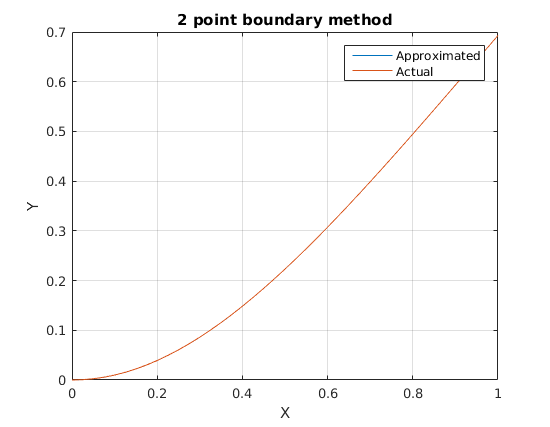
\includegraphics[scale = 0.55]{18_1.png}
    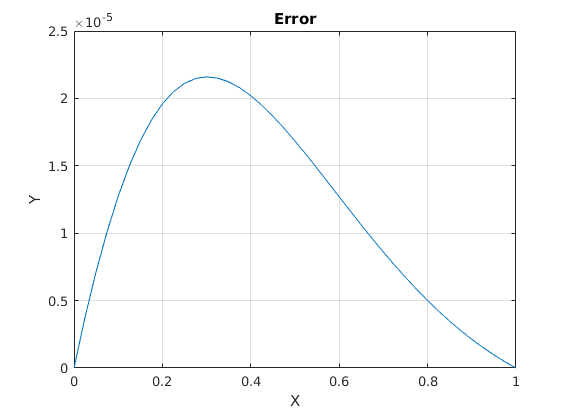
\includegraphics[scale = 0.55]{18_2.png}
    \caption{Comparison of Approximation}
\end{figure}

\end{document}